\def\QRCODE{MASTER_mispa_TUT.IMG.morphological_attribute_filtering_pythonqrcode.png}
\def\QRPAGE{http://www.iptutorials.science/tree/master/MASTER_mispa/TUT.IMG.morphological_attribute_filtering/python}
\pcorrectionsection{Python correction}

\begin{python}
from skimage import morphology as m
from scipy import misc
import matplotlib.pyplot as plt
from skimage.measure import regionprops
from skimage.measure import label
import numpy as np
\end{python}

\vspace*{-3pt}

\subsection{Binary attribute filtering}
If \pinline{bw} is a binary image, the different attribute are evaluated with \pinline{regionprops} and filtered according to the given upper and lower thresholds.

\begin{python}
def bwFilter(bw, attribute, thresholds):
    """
    binary filtering according to attribute
    bw: binary image
    attribute: string representing attribute, defined by regionprops
    thresholds: threshold values, inside which objects are removed
    returns binary image
    """    
    F = bw.copy();
    L = label(bw);
    for region in regionprops(L):
        a = getattr(region, attribute);
        if  a < thresholds[1] and a>= thresholds[0]:
            F[L==region.label] = False;
    return F;
\end{python}

\vspace*{-3pt}

\subsection{Grayscale filtering}
The grayscale filtering is the previous binary filtering process applied to all level-sets of the original image. 

\begin{python}
def grayFilter(I, attribute, thresholds):
    """
    grayscale image filtering by attribute
    for 8 bits unsigned images
    I: original grayscale image (N, M) ndarray
    attribute: string representing attribute, defined by regionprops
    thresholds: threshold values, inside which objects are removed
    returns grayscale filtered image
    """
    N, M = I.shape
    F = np.zeros((N, M, 256));
    for s in range(256):
        F[:,:,s] = s * bwFilter(I>=s, attribute=attribute, thresholds=thresholds);
    
    # reconstruction
    R = np.amax(F, axis=2);
    return R;
\end{python}

Then, for each level, the binary set is filtered by some attribute, and the resulting image is reconstructed by taking the maximum value on all levels.

The shape filtering process do not take the results from the \pinline{regionprops} function. The shape is filtered by using the morphological function of reconstruction.
\begin{python}
def shapeFilter(I, selem=m.square(25)):
    """
    image filtering when attribute is a shape of a given size, defined by selem
    I: grayscale image
    selem: structuring element
    returns: grayscale filtered image
    """
    N, M = I.shape
    F = np.zeros((N, M, 256));
    for s in range(256):
        F[:,:,s] = s * m.reconstruction(m.opening(I>=s, selem=selem), I>=s);
    
    # reconstruction
    R = np.amax(F, axis=2);
    return R;
\end{python}

The examples are generated via the following code:
\begin{python}
F = bwFilter(I>50, 'area', (0,5000));

F = grayFilter(I, 'area', (0,1000));

F = grayFilter(I, 'eccentricity', (0, 0.75));

F = grayFilter(I, 'solidity', (0, 0.75));

F = shapeFilter(I);
\end{python}

Results are illustrated in \iflabelexists{fig:morphological_attribute_filtering:enonce:examples}{Fig.\ref{fig:morphological_attribute_filtering:enonce:examples}.}{Fig.\ref{fig:morphological_attribute_filtering:python:examples}.
\begin{figure}[htbp]
\centering\caption{Attribute filtering examples.}%
\subfloat[Original image.]{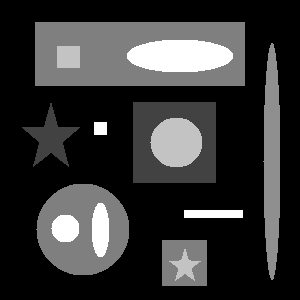
\includegraphics[width=.3\linewidth]{toy.png}}\hfill
\subfloat[Binary filtering by area (level 50 to get the binary image, 5000 pixels as a threshold).]{
\includegraphics[width=.3\linewidth]{toy_binary_areaOpening.python.png}}\hfill
\subfloat[Filtering by area (1000 pixels).]{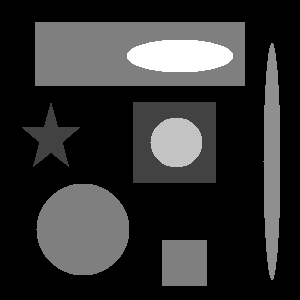
\includegraphics[width=.3\linewidth]{toy_areaOpening.python.png}}

\subfloat[Filtering by elongation ($0.75$).]{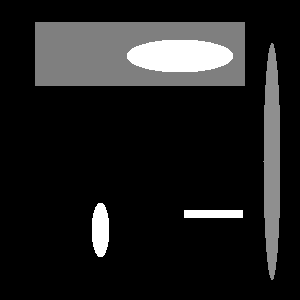
\includegraphics[width=.3\linewidth]{toy_elongThinning.python.png}}\hfill
\subfloat[Filtering by con\-ve\-xi\-ty ($0.75$).]{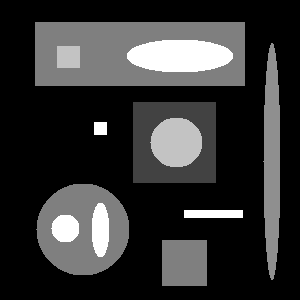
\includegraphics[width=.3\linewidth]{toy_convThinning.python.png}}\hfill
\subfloat[Filtering objects bigger than a square (of size $25\times 25$ pixels).]{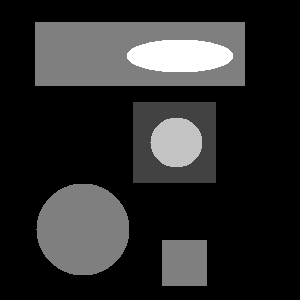
\includegraphics[width=.3\linewidth]{toy_recOpening.python.png}}%
\label{fig:morphological_attribute_filtering:python:examples}%
\end{figure}
}% iflabelexists

